% Theoretical background
%\clearpage%if the chapter heading starts close to bottom of the page, force a
% line break and remove the vertical vspace
\vspace{21.5pt}
\chapter{Analysis: Current vs. Proposed}
This chapter delineates a comprehensive study of the existing CI/CD pipeline
employed for embedded systems in the designated case company.
The focal point of the current analysis is the integration of diverse tools
with the Zephyr RTOS. A subsequent proposal for the pipeline's augmentation,
incorporating fuzzing, is presented with the aim of uncovering and
mitigating potential vulnerabilities, thereby enhancing the security and
dependability of the software solutions devised.

\section{Embedded System With Root Of Trust Architecture}
Reflecting on the prior discussions of embedded systems in
sections\ref{sec:sec_introduction} and\ref{sec:embedded_system} respectively,
this chapter explores current state analysis of the case in company and proposed
state of analysis with respect to fuzzing.

The figure:\ref{fig:rot} illustrates high-level depiction of the architecture for a
secure embedded system that leverages a Root of Trust (RoT) used in the company.

In an increasingly digital and interconnected world, the security of
embedded systems is paramount. Embedded systems, ranging from tiny
\gls{iot} devices to large-scale industrial control
systems, form the backbone of modern infrastructure. However,
their pervasiveness also makes them a tempting target for attackers. Vulnerabilities such as
Meltdown\cite{lipp2020meltdown} and Spectre\cite{kocher2020spectre} are some recent examples.
From data theft to device manipulation, the potential implications of
a successful attack are dire. Hence, there's a necessity for a robust
and secure foundation upon which these systems operate. This is where a secure architecture,
underpinned by a hardware \gls{rot}, becomes critical\cite{Introduc7:online}.

% \begin{figure}[ht]
%         \centering
%         \AltText{Embedded Root of Trust Architecture}{\includegraphics[width=9.5cm, height=10.5cm]{rot}}
%         \caption{Embedded Root of Trust Architecture}\label{fig:rot}
% \end{figure}

\begin{figure}[h]
        \centering
        \adjustbox{width=\textwidth}{\includegraphics{rot}}
        \caption{Embedded Root of Trust Architecture\cite{Introduc82:online}}\label{fig:rot}
\end{figure}

\textbf{Hardware:} This represents the physical components and sub-systems compromise
\gls{cpu}, memory\cite{WhatisCo30:online} and other peripherals. It acts as a base layer on which
rest of the system operates.

\textbf{Hardware Root of Trust:} Roots of Trust refer to secure components within a computer system,
encompassing hardware, software, or firmware\cite{WhatIsFi49:online}, that carry out crucial
security operations like data encryption, certificate validation and key management\cite{Hardware83:online}.
This is a principle that initiates a trust sequence, which is essential for verifying that
computers start up using authentic code. They serve as the foundational elements upon which the
security of other system components is established. Given their critical role, these elements must
be designed with a high level of
security\cite{WhatisRo39:online}\cite{Introduc7:online}\cite{RootofTr86:online}\cite{Hardware83:online}.

\textit{Hardware Root of Trust} ensures the integrity of the lower level system operations such as
secure boot\cite{zimmer2016establishing}, Debug and JTAG access control, Key management and Crypto Co-processors.
The \textit{secure boot} is a mechanism that the system uses to ensure that it ``boots'' in a known secure state.
The \acrshort{rot} plays a critical role in this process, verifying the integrity of the boot firmware and
subsequently loaded software\cite{Hardware83:online}\cite{zimmer2016establishing}.

The \textit{debug and JTAG access control} needs careful handling as it can be used maliciously although
an essential feature for debugging and troubleshooting purpose\cite{WhatisJT98:online}\cite{JTAGhard62:online}.

The \textit{device identity and key management} component helps in ensuring the use, storage
and generation of cryptographic keys. A unique identification is assigned to each device
in the system for authentication. Key management typically involves a \gls{hsm} for storage
of the keys\cite{WhatisKe81:online}. The keys are used for different operations such
as encryption\cite{WhatisEn13:online}, signing, and authentication\cite{needham1978using}.

The \textit{crypto core} is a component used in the \gls{rot} implementations
designed to be resistant to attack. This usually isolated from rest of the devices, helps
to protect the crypto core from being compromised. Some of the common cryptographic functions
are AES\cite{nechvatal2001report}, RSA\cite{milanov2009rsa}, and ECC\cite{bos2014elliptic}.

\textbf{Zephyr RTOS\cite{Security75:online}\cite{ZephyrPr4:online}\cite{ZephyrPr92:online}}
serves as a vital bridge between the hardware and application layers in an embedded system.
This compact, open-source Real-Time Operating System (RTOS) is thoughtfully engineered for devices
with resource limitations. Zephyr RTOS plays a critical role in facilitating the Root of Trust (RoT)
functionalities, such as secure boot, cryptographic procedures,
and device validation\cite{Security75:online}\cite{ZephyrPr4:online}\cite{ZephyrPr92:online}.

Key elements within the Zephyr RTOS include:
\begin{enumerate}
\item Device Drivers: The device drivers play a significant role in bringing the hardware
components, necessary for the Root of Trust, into operation. These hardware components
could be the cryptographic engine or the secure boot bootloader. Besides initialization,
these drivers make it possible for the kernel to manage and command these devices.
\item Kernel\cite{Kernelin72:online}: The kernel acts as the system's core, ensuring that only verified software is allowed
to boot up on the device. Its role is critical in maintaining the security condition
of the device, by managing processes, task scheduling, memory, and inter-process communication.
\item Middleware: This component offers a range of security services including secure storage
solutions for cryptographic keys and secure transmission protocols. It essentially forms a bridge
between applications and the underlying network services.
\item File System: The file system is employed to safeguard the security configuration
of the device, along with other classified information. Its main function is to prevent
unauthorized access or tampering with this sensitive data.
\end{enumerate}
Together, these components within the Zephyr RTOS form the backbone of a secure, robust RoT,
offering a trustworthy platform for all software operations within the system.

\textbf{Application Layer} includes the end-user applications, libraries, and
user interfaces. It interacts with the Zephyr RTOS to perform its operations. It provides the
important security features for the users.

\section{CI/CD for Embedded Software System}
In the context of the case in company, an integrated \gls{ci/cd} pipeline paired with the
Zephyr RTOS enhances the software development process. This integration leads to faster
firmware updates, better code quality, and more efficient development cycles.

Embedded systems, with their direct connections to hardware and real-world interactions,
require a specialized development approach. A robust \gls{ci/cd} pipeline is essential for
ensuring the reliability and efficiency of the software. This section provides a detailed
overview of the key stages in a \gls{ci/cd} flow.

\textbf{Development Environment and Version Control:}

Using a version-controlled codebase like Git\cite{loeliger2012version} ensures
an organized progression in the software development lifecycle. Gerrit\cite{milanesio2013learning},
used for hosting repositories, prompts a rigorous review for every code change,
which contributes to improved code consistency.

The figure:\ref{fig:CI_Infrastrcuture_1} illustrates IT Infrastructure for CI/CD flow for the
case in company.

% \begin{figure}[ht]
%         \centering
%         \AltText{Embedded CI/CD flow}{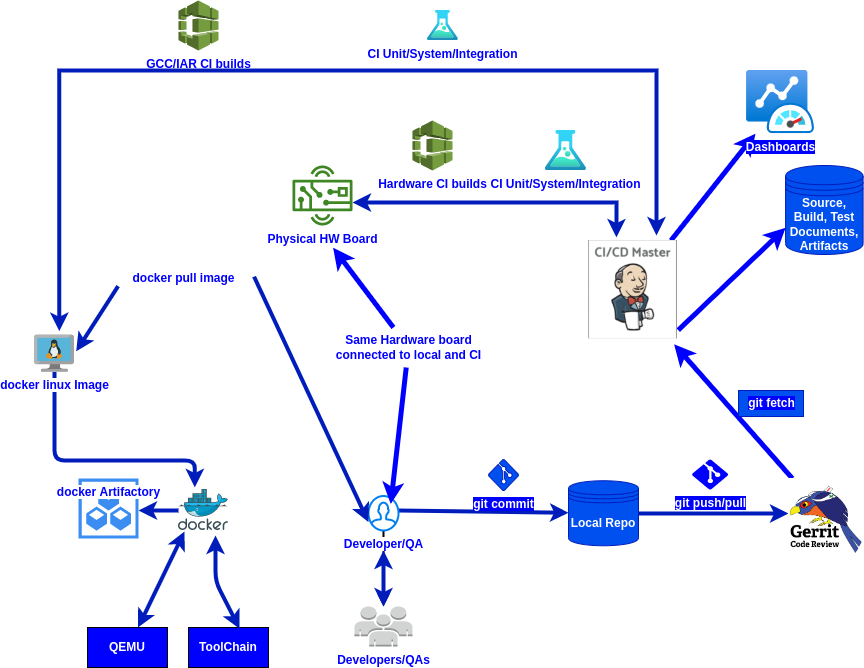
\includegraphics[width=10.5cm, height=15.5cm]{CI_Infrastrcuture_1}}
%         \caption{Embedded CI/CD flow}\label{fig:CI_Infrastrcuture_1}
% \end{figure}

\begin{figure}[h]
        \centering
        \adjustbox{width=\textwidth}{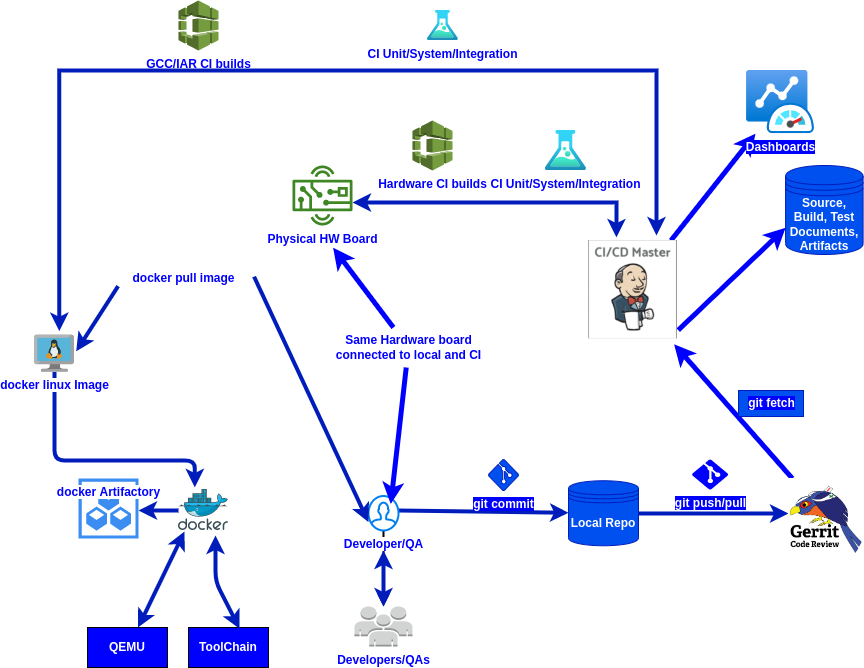
\includegraphics{CI_Infrastrcuture_1}}
        \caption{Embedded CI/CD flow}\label{fig:CI_Infrastrcuture_1}
\end{figure}

\textbf{Compilation Builds with GCC and IAR:}

For ensuring versatility and compatibility, multiple compiler configurations are essential.
The \gls{gcc} offers an extensive suite of software compilers
for various programming languages. It is widely recognized and utilized for its
efficiency and versatility\cite{GCCtheGN9:online}.
On the other hand, \gls{IAR} provides specialized compiler solutions for embedded systems,
ensuring optimal performance and reduced footprint, crucial for resource-constrained
devices\cite{AboutIAR98:online}.
Both these compilers are harnessed to guarantee that the Zephyr RTOS firmware
is compatible across diverse target platforms and meets the performance
requirements of embedded systems.

Automated processes compile the code after each modification. Tools like
\texttt{Clang Static Analyzer}\cite{kremenek2008finding} and \texttt{Coverity}\cite{imtiaz2019developers}
are then utilized for static analysis, detecting potential issues and inconsistencies.

\textbf{Using Docker\cite{anderson2015docker} for Environment Consistency and QEMU:}

Docker\cite{anderson2015docker} containers are used to maintain a consistent development environment
by packaging necessary dependencies for the Zephyr RTOS firmware compilation.
This approach reduces environmental discrepancies during builds.
\gls{QEMU}\cite{bellard2005qemu} serves as a hardware emulator, allowing for testing in a simulated
environment. This early-stage testing is crucial for detecting potential problems
before deployment to actual devices.

The docker image\cite{bui2015analysis} with the \acrshort{qemu} is pushed and saved in the
jfrog artifactory\cite{Artifact8:online} for the developers to use.

\textbf{Testing Frameworks:}

Ztest also called as Zephyr Test Framework which provides unit testing framework, which is applied to
validate the correctness of individual segments of the Zephyr RTOS code\cite{TestFram11:online}.

The Pytest\cite{hunt2019pytest} framework, checks the overall functionality and
interactions between the system's components. The Pytest framework works as system and
integration testing.

\textbf{Deployment and Continuous Monitoring:}

Jenkins, an established continuous integration tool\cite{smart2011jenkins}, orchestrates
an array of critical operations within the development workflow\cite{sayfan2017mastering}.
Upon each code submission to the repository, a cascade of processes is triggered.
This cascade encompasses code compilation, unit testing facilitated by the Ztest framework,
and system and integration testing conducted using the Pytest framework. Developers receive
prompt notifications of any anomalies detected during the build or testing phases.

The Jenkins interface provides comprehensive dashboards, detailing metrics such as
build failure instances and processing durations. Additionally, comprehensive reports are
archived for retrospective analysis. Continual monitoring after deployment is instrumental in
assuring the consistent and effective operation of the firmware.

\section{Proposed: CI/CD Pipeline with Fuzzing}
In light of the previously detailed CI/CD pipeline, it becomes imperative to
explore enhancements that could further fortify the software development
lifecycle. One such augmentation revolves around the incorporation of
fuzzing within the CI/CD pipeline, thereby aiming to unearth vulnerabilities
that conventional testing approaches might overlook.

Fuzzing, or fuzz testing, is a dynamic code testing technique that involves
injecting malformed or random data into a system to uncover vulnerabilities,
such as memory leaks, crashes, or other forms of unstable behaviors.
In the context of a CI/CD pipeline, integrating fuzzing translates to
routinely subjecting the developing software to a barrage of irregular inputs,
thereby aspiring to discern and rectify potential security vulnerabilities
before deployment.

\subsection{Integration into Existing Pipeline}
To assimilate fuzzing within the existing CI/CD pipeline, certain modifications
and additions are necessitated. Firstly, a fuzzing tool
compatible with the development environment needs to be selected.
Several robust, open-source fuzzing tools such as
AFL (American Fuzzy Lop) and LibFuzzer are available,
offering varying degrees of customization and coverage.

Once an appropriate fuzzing tool is elected, it is integrated into the CI/CD
pipeline, preferably at stages involving testing. Post the standard unit and
integration tests, the codebase is subjected to fuzz testing. This additional
layer of testing ensures that alongside verifying the correctness of code
functionalities and integrations, the robustness of the software against
malicious or unexpected inputs is also assessed.

\subsection*{Benefits and Challenges:}
The integration of fuzzing into the CI/CD pipeline brings forth several benefits.
Primarily, it enhances software security by proactively identifying and
addressing vulnerabilities, thereby reducing the risks associated with software
exploits. Additionally, it fosters the development of more resilient software,
as developers become cognizant of potential issues and refine their coding
practices accordingly\cite{HowCICDI34:online}.

However, this integration is not without its challenges. Fuzzing can be
resource-intensive, potentially prolonging the duration of the CI/CD pipeline.
Moreover, it might yield false positives, necessitating additional time and
resources to discern genuine vulnerabilities. Hence, a balanced approach,
where the depth of fuzzing is aligned with the project's criticality and
available resources, is essential\cite{FuzzingC40:online}.

\pagebreak
The figure:\ref{fig:CI_Infrastrcuture_fuzz_2} illustrates the proposed
IT Infrastructure for CI/CD flow for the case in company with fuzz testing.

\begin{figure}[H]
        \centering
        \adjustbox{width=\textwidth}{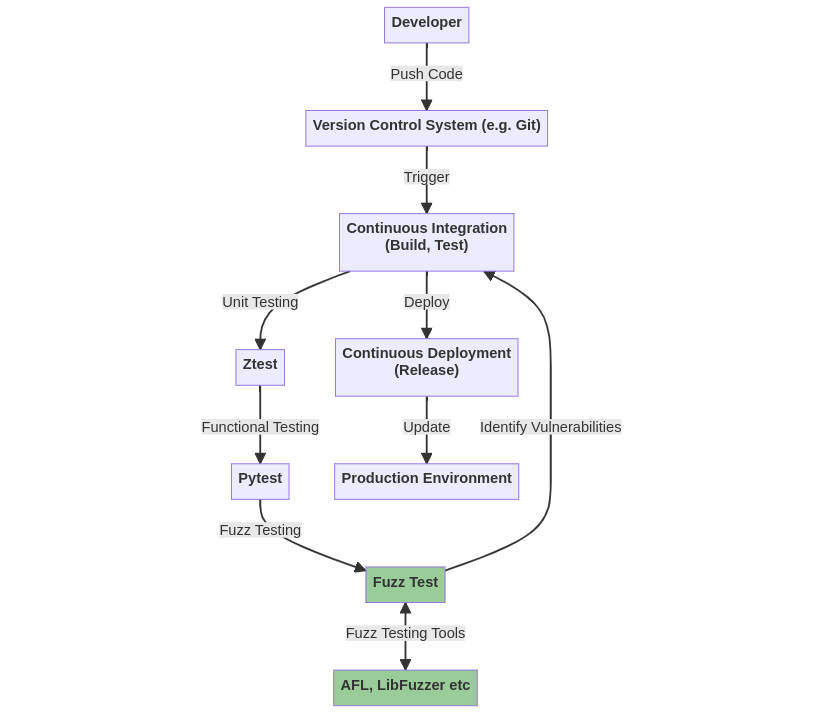
\includegraphics{CI_Infrastrcuture_fuzz_2}}
        \caption{CI/CD flow With Fuzz Testing}\label{fig:CI_Infrastrcuture_fuzz_2}
\end{figure}

\clearpage